tsets

%\documentclass[pra,twocolumn,epsfig,rotate,superscriptaddress,showpacs]{revtex4}


% \mathcal{u}se only LaTeX2e, calling the article.cls class and 12-point type.

\documentclass[prl,twocolumn,showpacs]{revtex4-1}
\usepackage{graphicx}
\usepackage{epsfig}
\usepackage{epsf}
\usepackage{amssymb}
\usepackage{amsmath}
\usepackage{amsthm}
\usepackage{multirow}
\usepackage{hyperref}

% \renewcommand{\familydefault}{\sfdefault}  %% arial font
% \usepackage{times} %% times new roman font

\newcommand{\bra}[1]{\langle #1|}
\newcommand{\ket}[1]{|#1\rangle}

\newcommand{\be}{\begin{equation}}
\newcommand{\ee}{\end{equation}}
\newcommand{\bea}{\begin{eqnarray}}
\newcommand{\eea}{\end{eqnarray}}
\newcommand{\Fig}[1]{Fig.\,\ref{#1}}
\newcommand{\Eq}[1]{Eq.\,(\ref{#1})}
\newcommand{\la}{\langle}
\newcommand{\ra}{\rangle}
\newcommand{\nl}{\nonumber \\}
\usepackage[usenames]{color}
\definecolor{Red}{rgb}{1,0,0}
\definecolor{Blue}{rgb}{0,0,1}






%%%%%%%%%%%%%%%%% END OF PREAMBLE %%%%%%%%%%%%%%%%



\begin{document}

% Include your paper's title here
\title{Experimental Estimation of Average Fidelity of a Clifford Gate on a 7-qubit Quantum Processor}
\author{Dawei Lu$^{1}$}
\author{Hang Li$^{1,2}$}
\author{Denis-Alexandre Trottier$^{1}$}
\author{Jun Li$^{1,3}$}
\author{Aharon Brodutch$^{1}$}
\author{Jonathan Baugh$^{1,4}$}
\author{Raymond Laflamme$^{1,5}$}
\email{laflamme@iqc.ca}


\affiliation{$^{1}$Institute for Quantum Computing and Department of Physics,
University of Waterloo, Waterloo N2L 3G1, Ontario, Canada}
\affiliation{$^{2}$Department of Physics, Tsinghua University, Beijing, 100084, China}
\affiliation{$^{3}$Department of Modern Physics, University of Science
and Technology of China, Hefei, Anhui, 230026, China}
\affiliation{$^{4}$Department of Chemistry, University of Waterloo, Waterloo N2L 3G1,
Ontario, Canada}
\affiliation{$^{5}$Perimeter Institute for Theoretical Physics, Waterloo, Ontario,
Canada}


\begin{abstract}
The traditional approach of characterizing a quantum gate via quantum process tomography requires an exponential number of experiments, which is impractical even for moderately large systems. In contrast, the twirling protocol is demonstrated to be able to tackle these problems efficiently, such as estimating the average fidelity of quantum memories and Clifford gates. Here, we certify an essential but complicated Clifford gate in a 7-qubit nuclear magnetic resonance quantum processor using the twirling protocol and sampling method. Under desired confidence level and confidence interval, the average fidelity of this Clifford gate in experiment is about 55\%, and rises to 87\% by eliminating the decoherence effect. The experiment spectrum related to this Clifford gate is also in great agreement with the simulated one. We state that reliable coherent controls in this system have been achieved in spite of the unavoidable decoherence. The entire protocol of certifying Clifford gates is efficient and scalable, as well as easily extended to other systems with minor modifications.
\end{abstract}
\pacs{03.67.Lx, 03.65.Wj, 03.67.Ac}

\maketitle



\paragraph*{Introduction.}

The methodology in characterizing the level of coherent control is fundamental and important in evaluating potential quantum information processing (QIP) devices. It provides a fair and intuitionistic comparison of controlling capabilities between diverse QIP devices, and also indicates the prospects of a designated system with respect to the fault-tolerant quantum computation \cite{Preskill1998}. The traditional approach by quantum process tomography (QPT) \cite{Chuang1997,Poyatos1997} is able to realize complete characterization of a quantum channel, and has been applied to utmost 3-qubit systems in experiment \cite{Childs2001,Weinstein2004,Brien2004,Riebe2006,Chow2009,Bialczak2010,Kim2014}. However, QPT suffers the exponentially amount of resources with the number of qubits growing, which results in the impracticality of its implementation even in relatively small systems. Moreover, in many cases full knowledge of a particular quantum gate is not necessary because some other physical descriptions of the gate are sufficient to reveal the noise level, while require much less experiments than QPT.  Several methods such as randomized benchmarking \cite{Emerson2005,Knill2008,Ryan2009}, twirling \cite{Emerson2007,Dankert2009,Moussa2012}, and Monte Carlo estimations \cite{Flammia2011,Silva2011} have been proposed to evaluate a particular quantum channel in an efficient manner, while all of them have their own restrictions and drawbacks. Here, in order to benchmark our coherent controls on a 7-qubit nuclear magnetic resonance (NMR) system, we adopted the twirling protocol \cite{Moussa2012} to estimate the average fidelity of an important Clifford gate in QIP. This gate enables the generation of the maximal coherence from single coherence with the aid of merely local rotations, and is indispensable in many QIP tasks such as creating the cat state in multi-qubit systems. The estimation method is scalable and independent of number of qubits, as well as easily implemented in other quantum computing architectures.

\paragraph*{Theory.}
For simplicity, let us consider the original twirling protocol for quantum memories \cite{Emerson2007}, where the quantum channel is a faulty identity $\Lambda$. The average fidelity of this noisy identity channel is defined as
\begin{align} \label{average_fidelity}
\bar{F}(\Lambda) = \int d\mu(\psi) \bra{\psi} \Lambda (\ket{\psi} \bra{\psi}) \ket{\psi},
\end{align}
where $d\mu(\psi)$ is the unitarily invariant distribution of pure states known as Fubini-Study measure \cite{Emerson2005}. Since a random state can be generated from a fixed state by applying a random unitary, we can equivalently average over a distribution of random unitaries invariant under conjugation
\begin{align} \label{average_Harr}
\bar{F}(\Lambda) = \int d\mu(\mathcal{V}) \bra{\psi} \mathcal{V}^{\dagger} \circ \Lambda \circ  \mathcal{V}(\ket{\psi} \bra{\psi}) \ket{\psi},
\end{align}
where $d\mu(\mathcal{V})$ is a unitarily invariant distribution of random unitaries known as Harr measure \cite{Emerson2005}.

After twirled over such Harr-distributed unitaries, $\Lambda$ will be reduced to a depolarizing channel, with the noise strength and average fidelity described by a single parameter \cite{Emerson2007}. However, it requires exponential number of  elementary gates to create a random Harr-distributed unitary, which makes the estimation of average fidelity inefficient. Fortunately, a unitary 2-design \cite{Dankert2009} such as the  Clifford group $\mathcal{C}$ is proved to be able to obtain an analytical expression of Eq. \ref{average_Harr}, by replacing the integral with a sum over the finite group
\begin{align} \label{average_Clifford}
\bar{F}(\Lambda) = \frac{1}{|\mathcal{C}|}\sum_{\mathcal{C}_i\in \mathcal{C}} \bra{\psi} \mathcal{C}_i^{\dagger} \circ \Lambda \circ \mathcal{C}_i(\ket{\psi} \bra{\psi}) \ket{\psi}.
\end{align}
In other words, averaging over $\mathcal{C}$ and averaging over Harr measure lead to the same average fidelity.

In particular, for a $n$-qubit system, $\mathcal{C}_1^{\otimes n}$ denotes the $n$-folder tensor product of the 1-qubit Clifford group, and its twirl transforms $\Lambda$ into a Pauli channel
\begin{align} \label{C1_twirl}
\bar{\Lambda}_{\mathcal{C}_1^{\otimes n}} = \frac{1}{|\mathcal{C}_1^{\otimes n}|}\sum_{\mathcal{C}_i\in \mathcal{C}_1^{\otimes n}} \mathcal{C}_i^{\dagger} \circ \Lambda \circ \mathcal{C}_i.
\end{align}
In fact, if terms are separated out according to their Pauli weight $w$, where $w$ is the number of non identity factors in the related Pauli operator, it can be shown that \cite{Silva2008}
\begin{align} \label{C1_twirlrho}
\bar{\Lambda}_{\mathcal{C}_1^{\otimes n}}(\rho) = \sum_{w=0}^n \text{Pr}(w) \left ( \frac{1}{3^w \binom{n}{w}} \sum_{i=1}^{3^w \binom{n}{w}} \mathcal{P}_{i,w} \rho \mathcal{P}_{i,w} \right ),
\end{align}
where $\text{Pr}(w)$ is the probability that a Pauli error of weight $w$ occurs. Furthermore, the average fidelity $\bar{F}(\Lambda)$ only depends on the probability of no error $\text{Pr}(0)$
\begin{align} \label{fidelity_pr}
\bar{F}(\Lambda) = \frac{2^n \text{Pr}(0) +1}{2^n +1}.
\end{align}
Thus the problem of estimating the average fidelity of $\Lambda$ is converted to the calculation of $\text{Pr}(0)$, which represents the probability of no error in $\bar{\Lambda}_{\mathcal{C}_1^{\otimes n}}(\rho)$.

To obtain $\text{Pr}(0)$, we can start from the input state $\ket{0}^{\otimes n}$, apply the $\mathcal{C}_1^{\otimes n}$ twirled channel, and measure the output state in the n-bit string basis \cite{Emerson2007}.  Equivalently, for an ensemble system we can replace $\ket{0}^{\otimes n}$ by $n$ distinct input states $\rho_w = Z^{\otimes w}I^{\otimes n-w}$, followed by a permutation operation $\Pi_n$, and measure accordingly as shown in Fig. \ref{everything}(a).

Moreover, O. Moussa \emph{et al.} proposed that \cite{Moussa2012} the original twirling protocol can be modified slightly if one wants to certify a faulty Clifford gate $\tilde{\mathcal{U}} = \mathcal{U} \circ \Lambda$. By inserting the identity $\mathcal{U}^{\dagger} \circ \mathcal{U}$ appropriately, the circuit depicted in the upper panel of Fig. \ref{everything}(a) will be transformed to the lower one.  Combinations of gates lead to a tremendously simple circuit, where the input state $\rho_{i} = \mathcal{C}_i \Pi_n \rho_{w} \Pi_n^{\dagger} \mathcal{C}_i^{\dagger}$ is the input Pauli operator spread over the entire Pauli group $\mathcal{P}_n$, and the measurement $M_{\rho_i, \mathcal{U}} = \mathcal{U} \rho_{i} \mathcal{U}^{\dagger}$ is also a Pauli operator. It is worth emphasizing that $M_{\rho_i, \mathcal{U}}$ can be calculated efficiently \cite{Aaronson2004}.

By implementing the circuit in the lower panel of Fig. \ref{everything}(a), the probability of no error is \cite{Alex2013}
\begin{align} \label{noerror}
\text{Pr}(0) = \frac{1}{4^n} + \frac{1}{4^n}\sum_{i=1}^{4^n-1} \text{Tr}\left( \tilde{\mathcal{U}} \left( \rho_{i}\right) M_{\rho_i, \mathcal{U}}\right).
\end{align}
Then substituting Eq. \ref{noerror} to Eq. \ref{fidelity_pr} will yield the average fidelity of the faulty Clifford gate $\tilde{\mathcal{U}}$.

Note that the above twirling protocol is limited to the certification of Clifford gates. For a general unitary gate, it is often impractical to realize the measurement operator $M_{\rho_i, \mathcal{U}} = \mathcal{U} \rho_{i} \mathcal{U}^{\dagger}$, whereas for a Clifford gate it can be pre-computed efficiently \cite{Aaronson2004}. Moreover, the Clifford gates are extremely significant as they construct elementary units in majority of fault-tolerant quantum computations based on stabilizer codes, and the universality is granted via magic state preparation \cite{Bravyi2005,Souza2011}. For instance, the encoding operation of the 3-qubit quantum error correction code is a Clifford gate comprising two controlled-NOT (CNOT) gates and a single qubit Hadamard gate, and has been certified in a 3-qubit solid-state NMR system \cite{Moussa2012}.

In spite of the tractability of the aforementioned way to estimate the average fidelity of Clifford gates, the complexity remains exponential as $4^n-1$ instinct Pauli states need to be prepared. Actually, measuring all of the expectation values is unnecessary if one only desires to approximate the average with a given confidence level and confidence interval. The Hoeffding's inequality \cite{Venkatesh2012} states that if $x_1, . . . ,x_m$ are independent realizations of a random variable $X$, confined to the interval $[a, b]$ and with statistical mean $\mathbb{E}(X) = \mu$, then for any $\delta >0$ we have
\begin{align} \label{Hoeffding}
\text{Prob} \left( |\bar{X}-\mu| > \delta \right) \leq 2e^{-2\delta^2m/(b-a)^2},
\end{align}
where $\bar{X} = \frac{1}{m}\sum_{i=1}^m x_i$ is the estimator of the exact mean $\mu$, and $\text{Prob}(\epsilon)$ denotes the probability of event $\epsilon: |\bar{X}-\mu| > \delta$ which we want to minimize apparently. Explicitly, the Hoeffding's inequality provides an upper bound to the probability that the estimated mean is off by a value greater than $\delta$. The confidence level and confidence interval are thus $1-\text{Prob}(\epsilon)$ and [$-\delta, \delta$], respectively.

Back to the estimation of the average fidelity, it is reasonable to set $a=0$ and $b=1$ as the bound of expectation values. Hence, for a given $\text{Prob}(\epsilon)$ and $\delta$, the number of experiments is
\begin{align} \label{exp_number}
m\leq \frac{\text{ln}(2/\text{Prob}(\epsilon))}{2\delta^2}
\end{align}
by taking natural logarithm of each side of Eq. \ref{Hoeffding}. Note that the number of experiments is independent of number of qubit $n$, once the desired $\text{Prob}(\epsilon)$ and $\delta$ have been given. This result reveals that the estimation of the average fidelity of Clifford gates via twirling protocol is efficient and scalable. For instance, given a $99\%$ confidence level, \emph{i.e.,} $\text{Prob}(\epsilon)=1\%$ and $\delta = 0.04$, the total number of experiments is 1656, regardless of whatever size of the system.

\begin{figure*}[htb]
\begin{center}
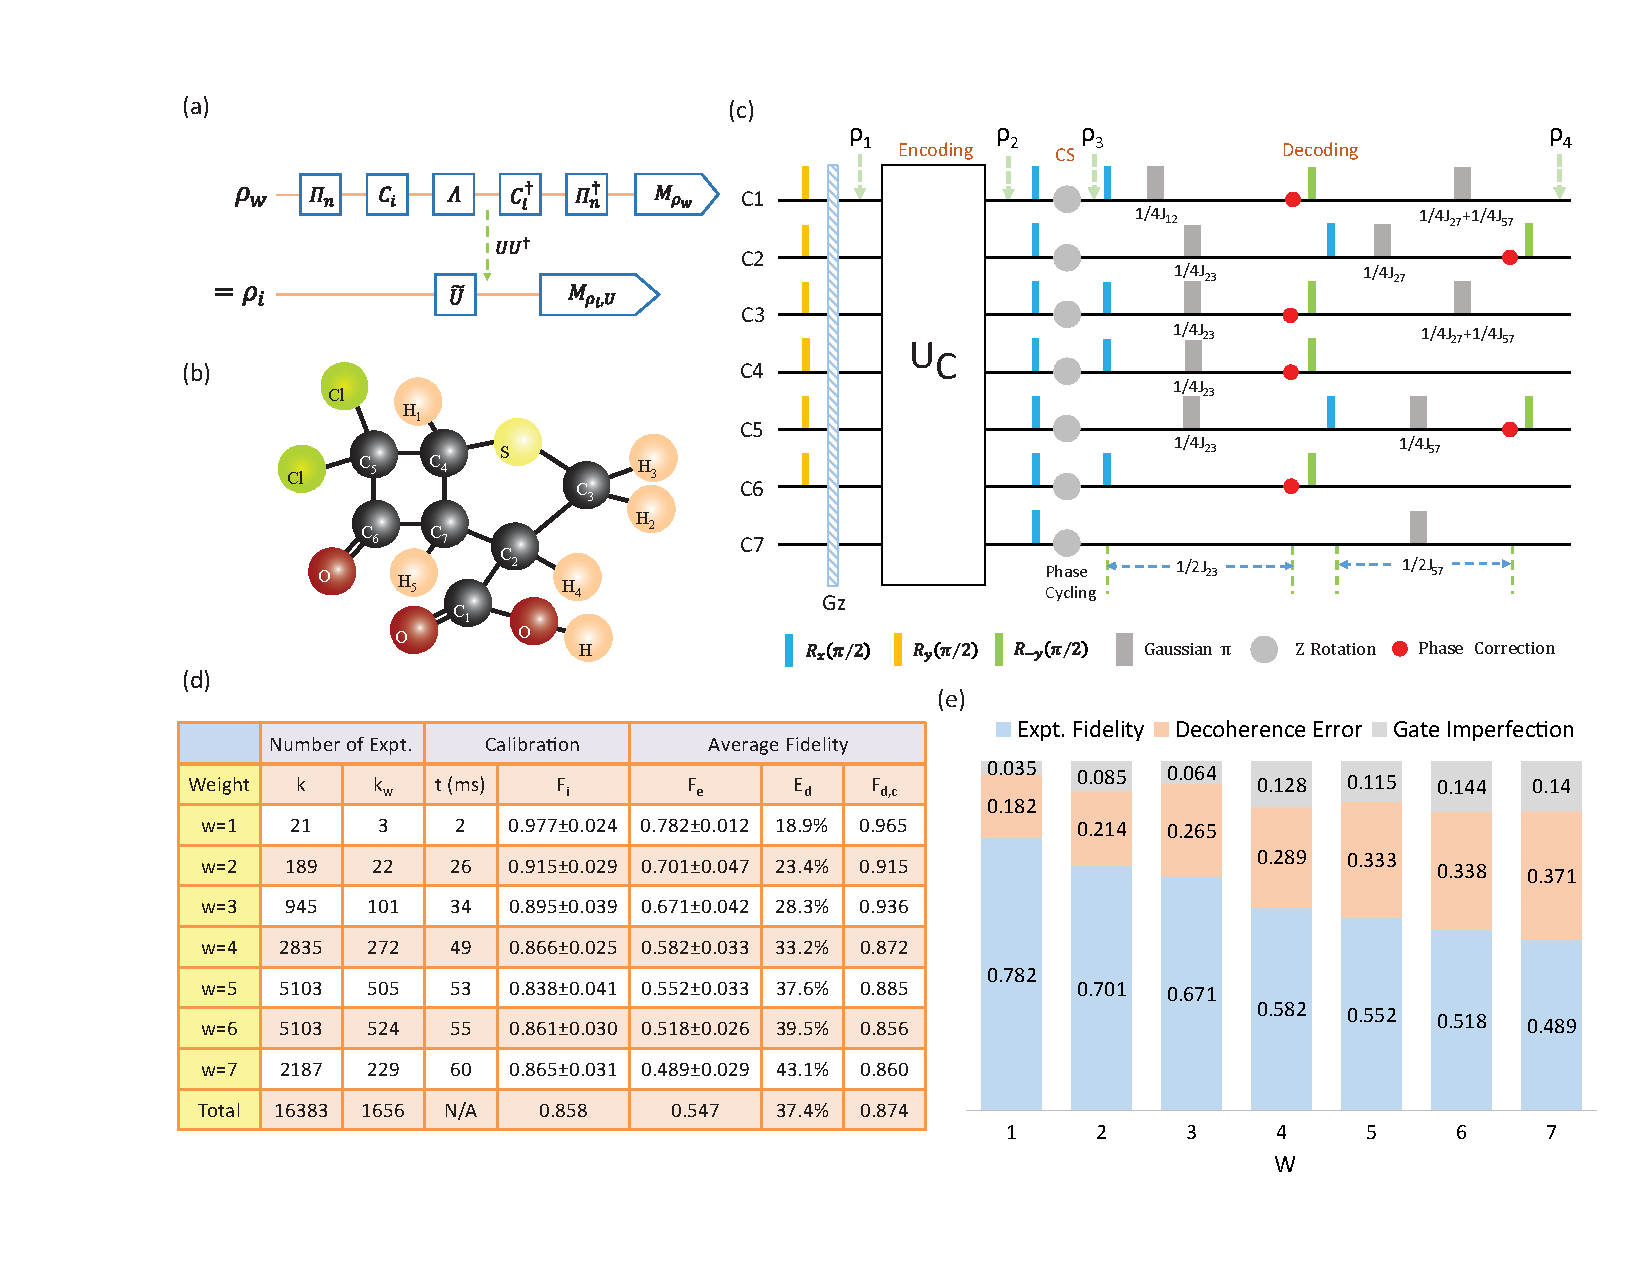
\includegraphics[width=2\columnwidth]{everything2.pdf}
\end{center}
\setlength{\abovecaptionskip}{-0.35cm}
\caption{\footnotesize{(color online). (a) Twirling protocols for quantum memories (upper) and Clifford gates (lower). Upper: $\rho_w = Z^{\otimes w}I^{\otimes n-w}$ represents $n$ distinct Pauli states, $\mathcal{C}_i$ is a 1-qubit Clifford operation in $\mathcal{C}_1^{\otimes n}$, and $\Pi_n$ is a permutation operation. Lower: $\rho_{i} = \mathcal{C}_i \Pi_n \rho_{w} \Pi_n^{\dagger} \mathcal{C}_i^{\dagger}$ spreads over the entire Pauli group $\mathcal{P}_n$, $\tilde{\mathcal{U}} = \mathcal{U} \circ \Lambda$ is the noisy Clifford gate, and $M_{\rho_i, \mathcal{U}} = \mathcal{U} \rho_{i} \mathcal{U}^{\dagger}$. (b) Molecular structure of Dichloro-cyclobutanone, where C$_1$ to C$_7$ form a 7-qubit system. (c) Pulse sequence for the creation of labeled PPS via the method in Ref. \cite{Knill2000}. It consists of three parts: encoding, coherence selection (CS) and decoding. $\mathcal{U}_{C}$, realized by a 80ms GRAPE pulse, is the Clifford gate to be certified. The instantaneous states are (unnormalized) $\rho_1 = I^{\otimes 6}\otimes Z$,  $\rho_2 = Z^{\otimes 7}$, $\rho_3 = \ket{0}\bra{0}^{\otimes 7}+\ket{1}\bra{1}^{\otimes 7}$, and $\rho_4 =  \ket{0}\bra{0}^{\otimes 6} \otimes Z_7$, respectively. (d) Experimental result for the certification of $\mathcal{U}_{C}$. $k=3^w\binom{7}{w}$ is the number of Pauli operators for weight $w$, while $k_w$ is the number of experiments via the sampling; $t$ is the typical time for the input Pauli state preparation, and $F_i$ is the calibration to capture the errors in preparation and measurement; $F_e$ is the experimental result of the probability of no error, and $F_{d,c}$ is the same quantity but without decoherence effect $E_d$. (e) Relationship among the experimental remaining signals (blue), decoherence effects (orange) and gate imperfections (gray) for different $w$.}}\label{everything}
\end{figure*}

\paragraph*{Experiment.}
The Clifford gate $\mathcal{U}_{C}$ to certify in our experiment was chosen as the the one to generate the maximal coherence from single coherence, up to a few local gates. It evolves $ZI^{\otimes n-1}$ to $Z^{\otimes n}$, and thus indispensable for the pseudo-pure state (PPS) preparation via the method proposed in Ref. \cite{Knill2000}, as the role of encoding process shown in Fig. \ref{everything}(c). Besides, it also serves as the essential operation for the creation of cat state $\left( \ket{0}^{\otimes n}+\ket{1}^{\otimes n} \right)/\sqrt{2}$ up to a certain number of phase gates. It can be decomposed into a sequence of elementary Clifford gates
\begin{align} \label{decomp}
e^{-i\frac{\pi}{2}I_x^i}e^{-i\pi I_z^i I_z^j} e^{-i\frac{\pi}{2}I_y^i},
\end{align}
which can increase the order of coherence by evolving $Z_i$ to $Z_i Z_j$. In addition, implementing this Clifford gate in experiment, \emph{e.g.} in NMR, is nontrivial as it requires $2(n-1)$ single qubit operations and $(n-1)$ 2-qubit operations, even regardless of refocusing gates inserted in the 2-qubit operations. Therefore, this Clifford gate is worthwhile to certify, for its significance in QIP and sufficiency in evaluating the level of coherent controls.

Our 7-qubit sample is $^{13}$C-labeled Dichloro-cyclobutanone dissolved in d6-acetone. The structure of the molecule is shown in Fig. \ref{everything}(b), where C$_1$ to C$_7$ denote the seven qubits. $^1$H nuclei were decoupled by the Waltz-16 sequence throughout all experiments. The internal Hamiltonian of this system can be described as
\begin{align}\label{Hamiltonian}
\mathcal{H}_{int}=\sum\limits_{j=1}^7 {2\pi \nu _j } I_z^j  + \sum\limits_{j < k,=1}^7 {2\pi} J_{jk} I_z^j I_z^k,
\end{align}
where $\nu_j$ is the resonance frequency of the \emph{j}th spin and $\emph{J}_{jk}$ is the scalar coupling strength between spins \emph{j} and \emph{k}. See supplemental material for the values of all parameters. All experiments were conducted on a Bruker DRX 700MHz spectrometer at room temperature.

The entire procedure to estimate the average fidelity of $\mathcal{U}_{C}$ can be divided into four parts, and the details are as follows.

(i) Sampling. To achieve a confidence level 99\% and precision $\delta = 0.04$, we computed that the required number of experiments is 1656 via Eq. \ref{exp_number}. Then we randomly sampled instinct 1656 Pauli states out of the entire 7-qubit Pauli group, which has in total $4^7-1=16383$ elements. We distributed all 1656 input Pauli states to seven subgroups according to their Pauli weights. The primary reason for this distribution is that a quantum gate such as $\mathcal{U}_{C}$ here is usually more vulnerable when applied to higher weight Pauli states. Additionally, the preparations of input Pauli states with different weight $w$ are distinct.

The sampling result is shown in Fig. \ref{everything}(d), where the number of sampled experiments $k_w$ for weight $w$ is around one tenth of the total number $k = 3^w\binom{n}{w}$.

(ii) Preparation and Calibration. For the creation of every input Pauli state, we employed the scalable sequence compiling program \cite{Ryan2008} to produce the corresponding pulse sequence. All pulses in the preparation sequences are local and generated by Gaussian shapes. Then we calibrated the preparation results aiming to capture the errors in preparation and measurements. The typical duration $t$ for preparing a weight $w$ Pauli state and the related calibration results $F_i$ are both listed in Fig. \ref{everything}(d).

(iii) Evolution. Our target operation $\mathcal{U}_{C}$ was optimized by the GRadient Ascent Pulse Engineering (GRAPE) pulse \cite{Khaneja2005}. Utilizing GRAPE algorithm guarantees that $\mathcal{U}_{C}$ is Clifford, as traditional state-dependent shape pulses for multiple qubits in NMR are hardly to form a strict Clifford operation. The GRAPE pulse of $\mathcal{U}_{C}$ was obtained with the pulse width chosen as 80ms and a theoretical fidelity 0.99, and then rectified in experiment to minimize the discrepancies between the ideal and implemented pulses \cite{Weinstein2004}.

(iv) Measurement. After applying the GRAPE pulse of $\mathcal{U}_{C}$ to each input Pauli state in experiment, we measured the corresponding output Pauli state by local readout pulses, and recorded the ratio of remaining signal.  Next we averaged the results with respect to different weight $w$, as shown by $F_e$ in Fig. \ref{everything}(d). It is reasonable that the ratio decreases substantially with $w$ increasing, as high coherent terms are extremely fragile to the decoherence occurring during the length of $\mathcal{U}_{C}$.

\begin{figure}[htb]
\begin{center}
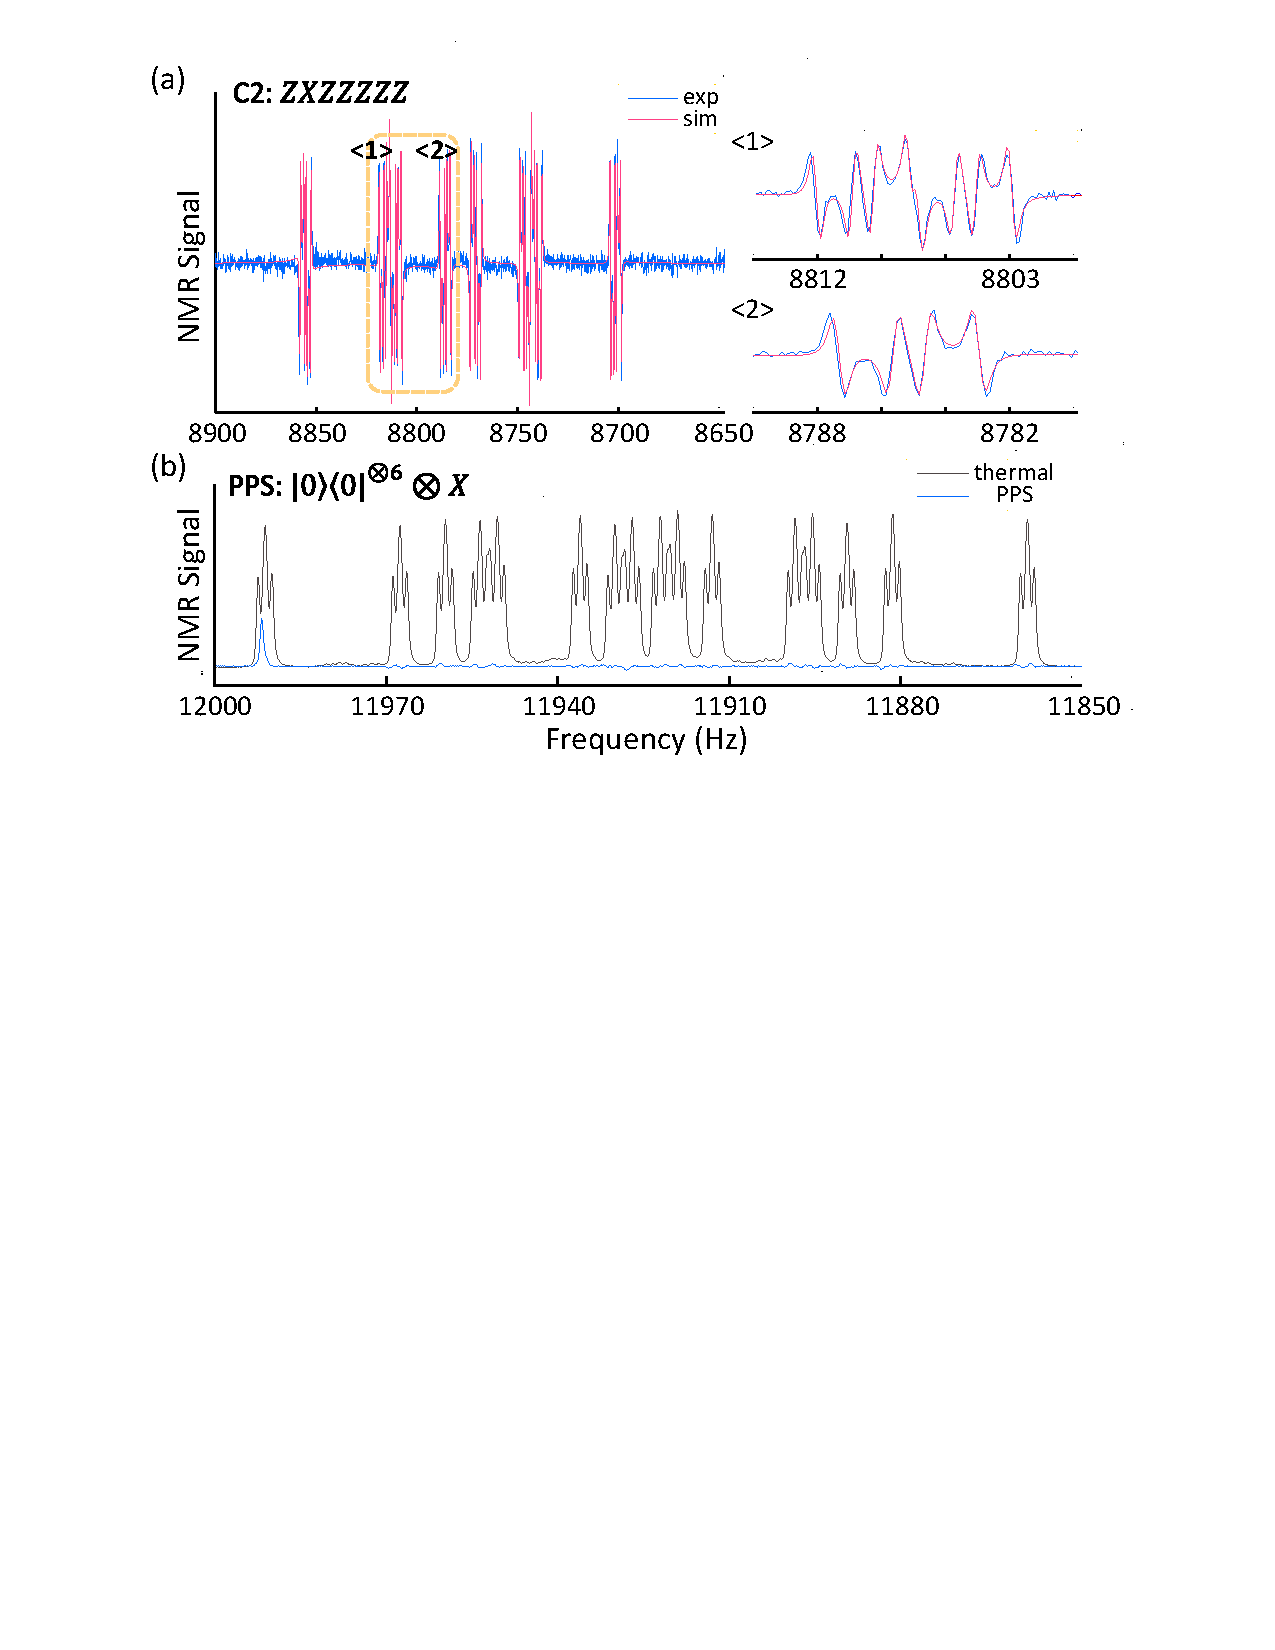
\includegraphics[width=\columnwidth]{spectra.pdf}
\end{center}
\setlength{\abovecaptionskip}{-0.35cm}
\caption{\footnotesize{(color online). (a) NMR spectrum of $Z^{\otimes 7}$ under the observation of C$_2$. The simulated (red) spectrum is re-scaled to achieve comprehensible comparison with the experimental (blue) one. (b) PPS spectrum (blue) based on the network in Fig. \ref{everything}(c), where $\mathcal{U}_{C}$ was employed as the encoding process. The spectrum of thermal equilibrium state (black) is also shown.}}\label{spectra}
\end{figure}

$F_e$ in Fig. \ref{everything}(d) illustrates that the probability of no error $\text{Pr}(0)$ is 54.7\%, meaning the average fidelity of $\mathcal{U}_{C}$ is about 55.1\% according to Eq. \ref{fidelity_pr}. Considering that  $\mathcal{U}_{C}$ roughly comprises twelve 1-qubit gates and six 2-qubit gates, the average error per gate is thus $\simeq 2.5\%$. To assess the decoherence effect in $\mathcal{U}_{C}$, we followed the approach of phase damping \cite{Vandersypen2001} to simulate the dynamical process step by step. The average signal attenuation due to decoherence is shown by $E_d$ in Fig. \ref{everything}(d). Under the assumption that the decoherence error is factorable, the probability of no error $\text{Pr}(0)$ after eliminating the decoherence is 87.4\%. Hence, compared to 55.1\% with decoherence, the average fidelity without decoherence rises to 87.5\%. So the average error per gate $\simeq 0.7\%$. which is mainly attributed to the imperfection in the designing and implementation of the GRAPE pulse.  Fig. \ref{everything}(e) displays straightforwardly the relationship among the raw experimental results, decoherence effects and gate imperfections for different $w$.

In Fig. \ref{spectra}(a) we also showed the spectrum of $Z^{\otimes 7}$ as the expected result of $\mathcal{U}_{C} Z_7 \mathcal{U}_{C}^{\dagger}$ under the observation of C$_2$. From the comparison between the simulated and experimental spectra, it convinces us that reliable coherent controls have been achieved in this 7-qubit system, in spite of the inevitable decoherence.  Moreover, we continued to prepare the labeled PPS based upon the network in Fig. \ref{everything}(c), where $\mathcal{U}_{C}$ was employed as the encoding process. The PPS spectrum by observing the labeled spin C$_7$ is shown in Fig. \ref{spectra}(b).

\paragraph*{Conclusion.}
In conclusion, we have shown how to efficiently estimate the average fidelity of a Clifford gate using the twirling protocol and random sampling method. In particular, we certified an important Clifford gate in a 7-qubit NMR quantum processor. To our knowledge, this is the largest gate-characterization in experiment to date. The results are in good accordance with the simulated ones, despite the unavoidable decoherence. Particularly, the experimental spectra based on this Clifford gate convinces us reliable coherent controls have been achieved in this 7-qubit system. Future work can be concentrated on the characterization of larger systems, or extension to other quantum systems.

We thank XXXXXXXXX for helpful comments and discussion. This work is supported by Industry Canada, NSERC and CIFAR.

\begin{thebibliography}{99}
\bibitem{Preskill1998} J. Preskill, Proc. R. Soc. A \textbf{454}, 385 (1998).
\bibitem{Chuang1997} I. Chuang and M. Nielsen, J. Mod. Opt. \textbf{44}, 2455 (1997).
\bibitem{Poyatos1997} J. Poyatos, J. Cirac, and P. Zoller, Phys. Rev. Lett. \textbf{78}, 390 (1997).
\bibitem{Childs2001} A. Childs, I. Chuang, and D. Leung, Phys. Rev. A \textbf{64}, 012314 (2001).
\bibitem{Weinstein2004} Y. Weinstein, T. Havel, J. Emerson, N. Boulant, M. Saraceno, S. Lloyd, and D. Cory, J. Chem. Phys. \textbf{121}, 6117 (2004).
\bibitem{Brien2004} J. O'Brien, G. Pryde, A. Gilchrist, D. James, N. Langford, T. Ralph, and A. White, Phys. Rev. Lett. \textbf{93}, 080502 (2004).
\bibitem{Riebe2006} M. Riebe, K. Kim, P. Schindler, T. Monz, P. Schmidt, T. K\"{o}rber, W. H\"{a}nsel, H. H\"{a}ffner, C. Roos, and R. Blatt, Phys. Rev. Lett. \textbf{97}, 220407 (2006).
%\bibitem{Chow2009} J. Chow, J. Gambetta, L. Tornberg, J. Koch, L. Bishop, A. Houck, B. Johnson, L. Frunzio, S. Girvin, and R. Schoelkopf, Phys. Rev. Lett. \textbf{102}, 090502 (2009).
\bibitem{Chow2009} J. Chow \emph{et al.}, Phys. Rev. Lett. \textbf{102}, 090502 (2009).
%\bibitem{Bialczak2010} R. Bialczak, M. Ansmann,	 M. Hofheinz,	E. Lucero, M. Neeley,	 A. O'Connell, D. Sank, H. Wang, J. Wenner,	M. Steffen,	A. Cleland, and J. Martinis, Nat. Phys. \textbf{6}, 409 (2010).
\bibitem{Bialczak2010} R. Bialczak \emph{et al.}, Nat. Phys. \textbf{6}, 409 (2010).
\bibitem{Kim2014} D. Kim \emph{et al.}, Nature \textbf{511}, 70 (2014).
\bibitem{Emerson2005} J. Emerson, R. Alicki, and K. Zyczkowski, J. Opt. B \textbf{7}, S347 (2005).
\bibitem{Knill2008} E. Knill \emph{et al.}, Phys. Rev. A \textbf{77}, 012307 (2008).
\bibitem{Ryan2009} C. Ryan, M. Laforest, and R. Laflamme, New J. Phys. \textbf{11}, 013034 (2009).
\bibitem{Emerson2007} J. Emerson \emph{et al.}, Science \textbf{317}, 1893 (2007).
\bibitem{Dankert2009} C. Dankert, R. Cleve, J. Emerson, and E. Livine, Phys. Rev. A \textbf{80}, 012304 (2009).
\bibitem{Moussa2012} O. Moussa, M. Silva, C. Ryan, and R. Laflamme, Phys. Rev. Lett. \textbf{109}, 070504 (2012).
\bibitem{Flammia2011} S. Flammia and Y. Liu, Phys. Rev. Lett. \textbf{106}, 230501 (2011).
\bibitem{Silva2011} M. Silva, O. Landon-Cardinal, and D. Poulin, Phys. Rev. Lett. \textbf{107}, 210404 (2011).
\bibitem{Silva2008} M. Silva, PhD thesis, University of Waterloo, 2008.
\bibitem{Aaronson2004} S. Aaronson and D. Gottesman, Phys. Rev. A \textbf{70}, 052328 (2004).
\bibitem{Bravyi2005} S. Bravyi and A. Kitaev, Phys. Rev. A \textbf{71}, 022316 (2005).
\bibitem{Souza2011} A. Souza, J. Zhang, C. Ryan, and R. Laflamme, Nat. Comm. \textbf{2}, 169 (2011).
\bibitem{Alex2013} D. Trottier, Master thesis, University of Waterloo, 2013.
\bibitem{Venkatesh2012} S. Venkatesh, \emph{The Theory of Probability: Explorations and Applications}. Cambridge University Press, 2012.
\bibitem{Knill2000} E. Knill, R. Laflamme, R. Martinez, C. Tseng, Nature \textbf{404}, 368 (2000).
\bibitem{Ryan2008} C. Ryan \emph{et al.}, Phys. Rev. A \textbf{78}, 012328 (2000).
\bibitem{Khaneja2005} N. Khaneja \emph{et al.}, J. Magn. Reson. \textbf{172}, 296 (2005).
\bibitem{Vandersypen2001} L. Vandersypen \emph{et al.}, Nature \textbf{414}, 883 (2001).
\end{thebibliography}


\end{document}
